\documentclass[]{article}

\usepackage{graphicx}
\usepackage[dutch]{babel}
\usepackage{fullpage}

\begin{document}

\title{Project Algoritmen en Datastructuren 3: \\Genetische Algoritmen en MPI}
\author{Jan Vermeulen}
\maketitle

\hrule

\section{Sequentiele Genetische implementatie}
\subsection{Beschrijving}

\subsubsection{Configuratie}
De sequenti\"ele implementatie kan geconfigureerd worden met de volgende extra parameters:
\begin{itemize}
\item Het aantal iteraties
\item De populatiegrootte
\item De maximale stap in x en y-richting bij mutatie
\item Het aantal crossovers
\item De kans op mutatie
\end{itemize}
De optimale parameters worden verder in dit verslag weergegeven.

\subsubsection{Initiele populatie}
Om een initiele populatie te genereren wordt de $n$-hoek opgedeeld in $n-2$ driehoeken, waarvan vervolgens de oppervlakte van berekend wordt.
Van deze oppervlakten wordt een cumulatieve array gevormd. Om een random punt te genereren op uniforme wijze wordt een getal tussen 0 en de som van de oppervlakten gegenereerd.
Aan de hand van de cumulatieve array en dit random getal selecteren we een driehoek. In deze driehoek met hoekpunten $P1$, $P2$ en $P3$ kiezen we een random punt (met $R1, R2 \in [0,1])$:\\[5pt]
\texttt{(1 - sqrt(R1)) * P1 + (sqrt(R1) * (1 - R2)) * P2 + (sqrt(R1) * R2) * P3}\\[5pt]
Dit wordt uitgevoerd voor elk punt in individu in de populatie.

\subsubsection{Datatypen}
De veelhoek wordt voorgesteld door een \texttt{struct} met een \texttt{integer} die het aantal hoeken bijhoudt, alsook een array van \texttt{float} types die de co\"ordinaten van de hoeken voorstelt.\\[5pt]
De \texttt{populatie} is slechts een array van \texttt{individu}en. Een individu wordt voorgesteld met een \texttt{struct} die de fitness en het aantal punten bijhoudt, alsook een array van \texttt{Point}s.\\[5pt]
Een \texttt{Point} is slechts een \texttt{struct} met 2 \texttt{float}s.

\subsubsection{Bepalen of punt binnen veelhoek ligt}
Om te bepalen of een punt P in de convexe veelhoek ligt worden de co\"ordinaten van de veelhoek verminderd met P in x en y-richting.
Vervolgens werd gebruik gemaakt van de volgende eigenschap:\\[10pt]
P ligt in veelhoek met punten $({x_0}, {y_0}), ({x_1}, {y_1}), ..., ({x_{n-1}}, {y_{n-1}}) \Leftrightarrow$\\
$ (\forall i \in [0,n-1]\ .\ x_{i+1 (mod\ n)}*y_{i}-x_{i}*y_{i+1 (mod\ n)} > 0) \vee \\(\forall i \in [0,n-1]\ .\ x_{i+1 (mod\ n)}*y_{i}-x_{i}*y_{i+1 (mod\ n)} < 0) $

\subsubsection{Crossover en mutatie}
Cross-over wordt uitgevoerd aan de hand van de opgegeven parameter \texttt{num\_crossovers}. Er worden dus in elke iteratie \texttt{num\_crossovers*2} kinderen gegenereerd.
Ook bij de mutatie wordt rekening gehouden met de parameters \texttt{max\_mutation\_step} (maximale stap in x en y-richting) en \texttt{mutation\_prob} (mutatiekans).

\subsubsection{Selectie}
In elke iteratie worden 2 selecties uitgevoerd. Als eerste worden ouders gekozen om kinderen mee te vormen. Na de mutatie van deze kinderen wordt nog een selectie uitgevoerd
waarin de individuen van de volgende populatie worden gekozen. Deze selectie wordt uitgevoerd met een techniek die stochastic universal sampling heet.\\

\noindent Initieel wordt een array opgebouwd met de cumulatieve fitness van alle individuen van de populatie.
Men kan dit visualiseren als volgt:
\begin{center}\includegraphics[width=400px]{SUS.png}\end{center}
Tussen 0 en de totale fitness wordt dan een willekeurige offset gekozen. Er wordt een afstand gedefinieerd
\begin{center}\texttt{distance = total\_fitness / n}\end{center}
waarbij $n$ het aantal elementen is dat je wil kiezen. Op deze manier worden individuen gekozen die op punten \texttt{offset+i*distance} op deze as liggen (met \texttt{i=0,1,...n}).
Punten met een grotere fitness hebben duidelijk een grotere kans om gekozen te worden.

\subsection{Testinput}
In de hieropvolgende metingen zal steeds gebruik gemaakt worden van de volgende convexe veelhoek:\\[10pt]
5\\
2.0 0.0\\
0.0 3.5\\
2.3 7.1\\
8.0 5.0\\
15.1 1.0\\
\begin{center}\includegraphics[width=300px]{polygon.png}\end{center}

\subsection{Evolutie van de fitness per generatie}
\begin{center}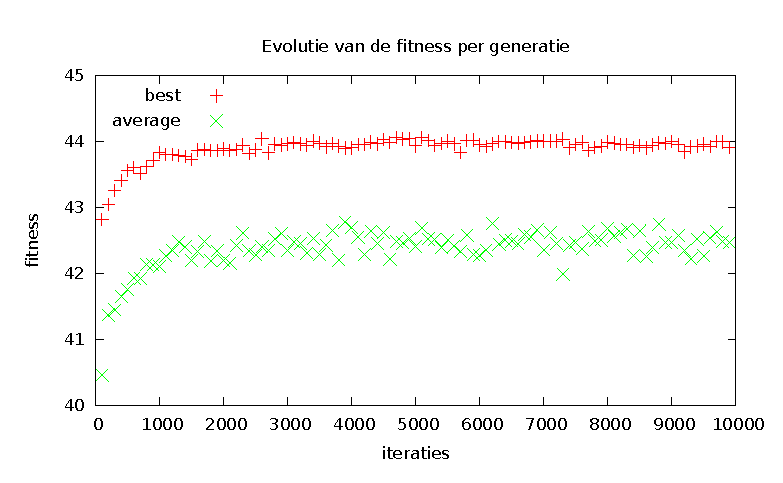
\includegraphics{plots/1_2.eps}\end{center}
Bij de eerste 300 iteraties stijgt de gemiddelde en beste fitness zeer snel. Naarmate de fitness het optimum nadert vertraagt deze stijging.
Vervolgens zien we een stagnatie met een licht stijgende trend. Voor deze meting werden de volgende parameters gebruikt:
\begin{itemize}
\item population\_size=200
\item max\_mutation\_step=0.9
\item num\_crossovers=100
\item mutation\_prob=0.5
\end{itemize}

\subsection{Invloed van de mutatiekans}
\begin{center}\includegraphics{plots/1_3.eps}\end{center}
Hoewel voor deze meting gemiddelden van 30 uitvoeringen werden beschouwd, is er niet echt een algemene trend af te lezen uit deze data.
De hoogste fitness werd in deze metingen bereikt met een mutatiekans van 0,75. Er lijkt echter geen sterk verband te zijn tussen de mutatiekans en de fitness van het beste individu na n iteraties voor deze implementatie.
Voor deze meting werden de volgende parameters gebruikt:
\begin{itemize}
\item iterations=3000
\item population\_size=200
\item max\_mutation\_step=0.9
\item num\_crossovers=100
\end{itemize}

\subsection{Invloed van de populatiegrootte}
\begin{center}\includegraphics{plots/1_4.eps}\end{center}
Het is duidelijk dat de beste fitness van de populatie zal stijgen naarmate de populatie groter wordt. De fitness stijgt initieel zeer snel, maar de stijging zwakt zeer snel af.
De grafiek heeft een verloop gelijkaardig aan een logaritmische functie.
Voor deze meting werden de volgende parameters gebruikt:
\begin{itemize}
\item iterations=3000
\item max\_mutation\_step=0.9
\item num\_crossovers=100
\item mutation\_prob=0.3
\end{itemize}

\subsection{Invloed van het aantal crossovers}
\begin{center}\includegraphics{plots/1_5.eps}\end{center}
Tegen de intu\"itieve verwachting in, zien ze een daling van de beste fitness naarmate het aantal crossovers (equivalent met het aantal kinderen maal 2 in elke iteratie) te groter wordt.
Het aantal crossovers mag dus niet te groot gekozen worden.
Deze meting werd uitgevoerd met volgende parameters:
\begin{itemize}
\item iterations=3000
\item population\_size=500
\item max\_mutation\_step=0.9
\item mutation\_prob=0.3
\end{itemize}


\subsection{Invloed van de maximum stap bij mutatie}
\begin{center}\includegraphics{plots/1_6.eps}\end{center}
Bij een heel kleine maximum stap, zien we een zeer sterke stijging in de grafiek. Nadat deze curve een lokaal optimum bereikt,
zien we een zeer kleine daling. De maximum stap kiezen we dus best niet te klein. Het optimum wordt hier ongeveer bereikt in 0,6.
Deze meting werd uitgevoerd met volgende parameters:
\begin{itemize}
\item iterations=3000
\item population\_size=500
\item num\_crossovers=200
\item mutation\_prob=0.3
\end{itemize}

\subsection{Performantie en geschiktheid}
\begin{center}\includegraphics{plots/1_7.eps}\end{center}
Aangezien dit algoritme iteratief is, heeft dit logischerwijs een lineaire complexiteit. Een genetisch algoritme lijkt zeer geschikt om dit probleem op te lossen,
aangezien een optimale plaatsing slechts kan bekomen worden door trial and error. Een genetisch algoritme lijkt de enige mogelijkheid om dit probleem op te lossen
in lineaire tijd. Het is mogelijk om de huidige parameter van het aantal iteraties te vervangen
door een nauwkeurigheid en vervolgens het algoritme stop te zetten wanneer de verbetering van de fitness kleiner is dan de nauwkeurigheid.

\section{Gedistribueerd algoritme}
\subsection{Beschrijving}
Het parallel algoritme heeft nog 1 extra parameter, namelijk het aantal synchronisaties.
Bovenop een aantal iteraties zal dit algoritme om de n iteraties synchroniseren en zal elke thread zijn individuen uitwisselen met
andere threads.  Hieronder staat een voorbeeld met N iteraties en 2 synchronisaties.
\begin{center}\includegraphics[width=400px]{synchs.png}\end{center}
Deze synchronisatie gebeurt met \texttt{MPI\_Alltoall}. Indien er n processen zijn, worden de individuen van elke thread opgedeeld in groepen van
\texttt{population\_size/n}. De i-de groep individuen van het elk proces zal vervolgens terechtkomen bij het in i-de proces.
Om de uitwisseling van individuen tussen threads mogelijk te maken, wordt de populatie individuen omgezet naar een array van \texttt{float}s.\\
Na afloop van alle iteraties en synchronisaties wordt het individu met beste fitness gekozen in elk proces. Dit wordt dan vergeleken met de
beste individuen van alle andere processen met behulp van \texttt{MPI\_Allreduce} met \texttt{MPI\_MAXLOC}.

\subsection{Verhouding aantal synchronisaties en aantal iteraties}
Het totale aantal iteraties is equivalent met het product van de parameters \texttt{synchs} en \texttt{iterations}. 
Bij volgende testen werd dus steeds \texttt{iterations} verlaagd wanneer \texttt{synchs} verhoogd werd, zodat we hetzelfde
aantal effectieve iteraties behouden, met meer synchronisatiestappen tussen de iteraties.
\begin{center}\includegraphics{plots/2_2.eps}\end{center}
Ook hier kan geen sterke correlatie aangetoond worden, maar we zien wel een stijging naarmate het aantal synchronisaties verhoogd wordt.
Deze meting werd uitgevoerd met volgende parameters:
\begin{itemize}
\item population\_size=200
\item max\_mutation\_step=0.5
\item num\_crossovers=100 
\item mutation\_prob=0.75
\end{itemize}

\section{Performantievergelijking}
Om een vergelijking te maken tussen het sequentieel en het parallel algoritme werd de parameter \texttt{iterations} van de parallelle implemetatie
constant gehouden. Na 50 iteraties werd dus steeds een synchronisatie uitgevoerd. Het aantal iteraties uit de sequenti\"ele versie kwam dus steeds overeen met
\texttt{synchs*iterations} van de parallelle versie.
\begin{center}\includegraphics{plots/2_3.eps}\end{center}
Tijdens de eerste 1500 iteraties loopt het parallel algoritme ongeveer gelijk aan het sequentieel algoritme. Dit is te wijten aan de overhead van MPI.
Vervolgens zien we dat het parallel algoritme steeds een kleinere uitvoeringstijd kent vergeleken met het sequenti\"ele algoritme.\\
Deze meting werd uitgevoerd met volgende parameters:
\begin{itemize}
\item population\_size=50
\item max\_mutation\_step=0.5
\item num\_crossovers=200 
\item mutation\_prob=0.3
\end{itemize}



\end{document}